\documentclass[a4paper,10pt]{article}
%\documentclass[a4paper,10pt]{scrartcl}

\usepackage[utf8x]{inputenc}
\usepackage[brazil]{babel}
\usepackage{graphicx}
\usepackage{float}
\usepackage{scalefnt}

\begin{document}

\begin{titlepage}
\vfill
\begin{center}
{\Large Universidade Federal do Rio de Janeiro} \\[7cm]
{\Large \textbf{Simulação de Filas}}\\[5cm]
\begin{large}{Trabalho de Avaliação e Desempenho - MAB 515 \\ Professor:Paulo Henrique de Aguiar Rodrigues}\end{large}
\vfill
{RIO DE JANEIRO\\2011}
\end{center}
\end{titlepage}

\begin{titlepage}
\textbf{Integrantes e suas Participações:}
\begin{itemize}
 \item Diego Fonseca Pereira de Souza   DRE:108055513
 \begin{itemize}
    \item Assinatura: \rule{6cm}{.1mm}	
    \item Participação:
    \begin{itemize}
	\item Obtenção de Resultados
	\item Confecção do Relatório
	\item Confecção dos Gráficos
	\item Teste de Validação
	\item Otimização
	\item Análise de Resultados
    \end{itemize}
 \end{itemize}
 \item Ewerton Vinicius Ramos Balthazar DRE:106044875
  \begin{itemize}
    \item Assinatura: \rule{6cm}{.1mm}	
    \item Participação:
    \begin{itemize}
	\item Obtenção de Resultados
	\item Confecção do Relatório
	\item Teste de Validação
	\item Otimização
	\item Análise de Resultados
    \end{itemize}
 \end{itemize}
 \item Gustavo Rodrigues Lima           DRE:108055416
  \begin{itemize}
    \item Assinatura: \rule{6cm}{.1mm}	
    \item Participação:
    \begin{itemize}
	\item Implementação do Simulador
	\item Depuração Do Simulador
	\item Confecção do Relatório
	\item Teste de Validação
	\item Estimativa da fase transiente
	\item Estimativa de tamanho e número de rodadas
    \end{itemize}
 \end{itemize} 
 \item Gustavo Daniel Soares Figueiredo DRE:106051068 
  \begin{itemize}
    \item Assinatura: \rule{6cm}{.1mm}	
    \item Participação:
    \begin{itemize}
	\item Implementação do Simulador
	\item Depuração Do Simulador
	\item Confecção do Relatório
	\item Teste de Validação
	\item Estimativa da fase transiente
	\item Estimativa de tamanho e número de rodadas
    \end{itemize}
 \end{itemize} 
\end{itemize}
\end{titlepage}

\pagestyle{plain}

\section{Apresentação do Problema}
   Executar uma simulação do comportamento de um sistema no qual duas filas disputam o servidor e umas das filas tem prioridade preemptiva sobre a outra.
   \begin{figure}[H]
      \center
      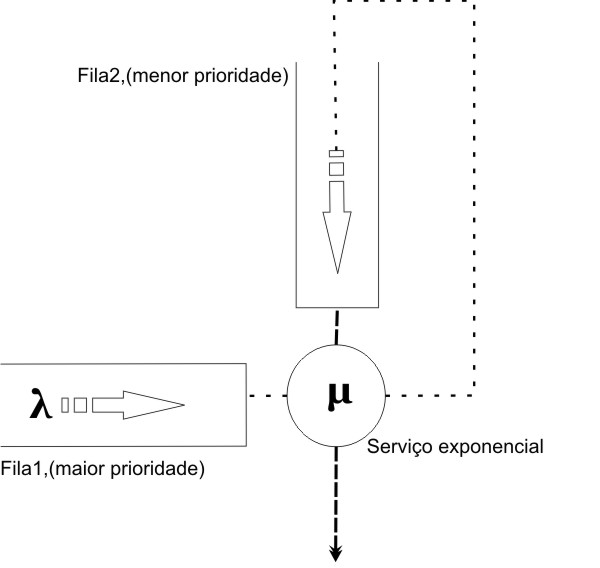
\includegraphics[scale=3]{AD-Relatorio.jpg}
      \caption{Esquema do sistema}
  \end{figure}
  Fregueses chegam à fila 1 segundo um Processo Poisson com taxa $\lambda$ (tempo entre chegadas é exponencial com taxa $\lambda$).Esta é a fila de maior prioridade do sistema.Após
  serem servidos pela primeira os fregueses seguem para a fila 2 , de menor prioridade .Ao término deste segundo serviço, os fregueses vão embora.Tanto o primeiro como o segundo 
  serviços do freguês são obtidos de forma independente a partir de uma distribuição exponencial com taxa $\mu=s^{-1}$.Isto significa que os serviços
  recebidos por um mesmo freguês são totalmente independentes.Todavia,o serviço em andamenteo da fila 2 pode ser interrompido ,pela chegada de um freguês na fila 1.Neste caso, o serviço
  interrompido será retomado de onde parou.Observe que um freguês da fila 2 poderá ser interrompido mais de uma vez.As filas operam sobre o regime \textbf{FCFS} (First Come First Servide -
  o primeiro à chegar é o primeiro à ser servido).
\section{Solução Proposta}
      \subsection{Introdução}
	\subsubsection{Funcionamento Geral do Simulador}
	Quando o programa é inicializado, ele chama a classe Simulador esta chama a ManipulaXML que farará a leitura do xml, este arquivo contém os parâmetros que podem ser alterados do programa , como o tamanho da fase transiente
	número de rodadas , tamanaho da rodada, disciplina de atendimento , utilização e taxa de serviço.Após a leitura do xml a classe Simulador cria o "loop" principal do programa, baseado no número de rodadas , a cada rodada ela chama 
	a classe Rodada que cria  as filas de acordo com a disciplina especificada.A partir desse momento começa-se a gerar os eventos de chegada e saída do programa , mas para fazer isso fazemos uso da Classe Gerenciado de Eventos.O objetivo
	da classe GerenciadorEventos é gerar os eventos e dizer qual é o próximo evento a ser tratado , caso o próximo evento seja de chegada e o seridor não esta ocupado o novo freguês vai direto para o serviço , no nosso sistema a classe Servidor
	que realiza o serviço, caso o servidor esteja ocupado com um freguês oriundo fa fila 2, o mesmo é retirado do servidor e reposicionado na fila com o tempo de serviço residual preenchido , o último caso possível é quando quem está em serviço
	é um frêgues da fila 1 , logo o novo cliente terá de ficar esperando na fila.
 	\subsubsection{Os Eventos Escolhidos}
	O sistema possui três eventos:\\
	Chegada$\to$ Ocorre quando um cliente chega no sistema, ou seja um novo freguês entra na fila 1 ou direto para serviço \\
	Saida$\to$ Ocorre quando um cliente sai da sua fila e vai para o servidor,se o freguês vem da fila 1, quando acabar de ser sevido vai para a fila 2 , caso seja da fila 2 irá embora do sistema.\\
	Interrupção$\to$ Quando ocorre um evento de chegado no sistema e quem está em serviço  é um freguês da fila 2, efetivamente não um evento de interrupção, porque depois de tratado virá um evento de saida.O que fazemos 
	é devolver o clinte interrompido para sua fila e colocar o tempo de serviço residual em um variável.\\
	\subsubsection{Método usado:replicativo}
	Este método se configura da seguinte forma: a cada rodada de simulação usa-se uma nova semente.Deve ter bastante cuidado com a estimativa da fase transiente e ter sementes bastante distantes uma das outras para se evitar qualquer
	dependência estocástica entre as medidas.Para gerar semente nos chamamos a classe Math do java e pedimos para ela gerar um número aletório , após isso multiplicamos por um número muito grande para aumentar a probabilidade de sempre 
	termos sementes distintas, com a semente gerada pegamos a mesma e passamos como parâmetro para classe Random do java, para agora sim podemos gerar nosso eventos.
	\subsubsection{Geração da variáveis aleatórias}
	Para gerar as variáveis aleátorias fazemos uso da seguinte fórmula $x_0 = -\frac{\ln u_0}{taxa}$, onde $u_0$ é gerado aleatoriamente pela classe GeradorAleatório e a taxa depende para qual evento estamos querendo gerar uma amostra.
	Caso seja para um evento de saida usaremos $\mu$ que representa a taxa de serviço.Já se for evento de chegada usaremos $\lambda$, que é a taxa com que os fregueses chegam ao sistema , este valor pode ser obtido pela seguinte fórmula:
	$\rho = 2\lambda$, onde $\rho$ representa a utilização do sistema que é informado no arquivo de configuração.
	\subsubsection{Escolha dos Parâmetros}
	\subsubsection{Implementação do Conceito de Cores}
	O método replicativo gera uma facilidade na implementação das cores, basta apenas dizer se o freguês faz ou não parta da fase transiente.Criamos um "enumerator", faz com um variável possa apenas possa assumir os valores informado no 
	"enumerator", que no nosso caso será "TRANSIENTE" ou "NAOTRANSIENTE" dessa forma implementamos o conceito de cores.A diferença entre a marcação é que quando  marcamos um cliente como "TRANSIENTE" ele não será levado em consideração 
	no cálculo estatístico.A fase transiente sever basicamente para colocar o sistema em equilíbrio.
	\subsubsection{Estrutura Interna Utilizada}
	As estruturas utilizadas para representar as filas foram as seguintes , para as com disciplina de atendimenteo FCFS (First Come First Servide) fazemos uso de uma fila e sempre inserimo um novo cliente no final, quando o servidor está
	desocupado e tem cliente na fila pegamos o primeiro da fila.Já a disciplina LCFS(Last Come First Servide) colocamos o cliente no inicio da fila , se o servidor está vazio e tem freguês na pilha colocamos o primeiro da pilha em serviço.
	\subsubsection{Equimamentos de Teste}
	O equipamento utilizado nos teste foi o seguinte:
	\begin{itemize}
	 \item  Processador: i5 - Modelo 760 - Clock de 2,8 Ghz
	 \item  Memória: 2x2GB DDR3 - Modelo:KVR1333D3N9 - Trabalhando em Dual Channel 
	 \item  Placa-Mãe: Gigabyte - Modelo:P55-USB3
	 \item  Sistema Operacional: Windows 7 Professional 64 bits
	\end{itemize}
	\subsubsection{Linguagem Utilizada}
	A linguagem escolhida foi o Java , devido ao maior dominio dos integrantes do grupo nesta linguagem e também pelas estruturas de alta performance já implementadas.
	\subsubsection{Outra Informações Pertinentes}
	\begin{enumerate}
	 \item Para poder rodar o programa,se for o windows criamos o arquivo simulador.bat  que tem internamente o comando para rodar o arquivo .jar ,gerado do código do programa, caso seja linux criamos o simulador.sh.
	 \item O programa pode tratabalhar tanto com a disciplina de atendimenteo FCFS ou LCFS.
	 \item Para não precisar ir ao código para trocar os parâmetros de entrada nos criamos um arquivo chamado config.xml que fica dentro da pasta XML, este arquivo sempre será lido quando se inicia o simulador , caso não seja 
	  possível localizar o arquivo, a simulação será realizada com os parâmetros padrão especificado no código.
	  \begin{figure}[H]
	      \center
	      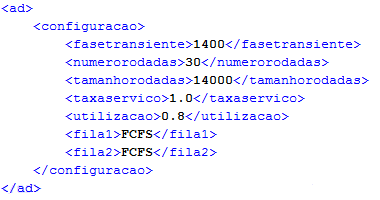
\includegraphics[scale=0.75]{Capturar.PNG}
	      \caption{Exemplo do config.xml}
	  \end{figure}
	  Explicação de cada tag:\\
	  fasetransiente$\to$Determina a quantidade de chegadas(Fregueses) que não terão estatísica  computada no início de cada rodada. O objetivo é que o sistema alcance o equilíbrio para ter maior exatidão mo cálculo estatístico.\\
	  numerorodadas$\to$Determina quantas rodadas serão simuladas, computando as estatísticas ao final de cada uma delas.\\
	  taxaservico$\to$Taxa com que o servidor ira atender os fregueses.\\
	  tamanho da rodada$\to$Número total de chegadas que ocorrerão e serão tratadas pelo sistema em uma rodada.
	  utilizacao$\to$taxa que indica a utilizacao do sistema ou seja $\rho$.\\
	  fila1 e fila2$\to$indica a disciplina de atendimenteo na fila 1 e 2, respectivamente.Podendo ser FCFS ou LCFS.\\
	\end{enumerate}

      \subsection{Teste de Correção}
      Para verificar a correção do simulador usaremos de dois casos básicos:
      \begin{itemize}
	 \item Quando ocorre uma única chegada no sistema:
	 \item Quando o cliente chega ao sistema e encontra fregueses na fila 1, 2 e fregueses sendo servidos;
      \end{itemize}
      Vamos descrever passo a passo o comportamento esperado do simulador e, em seguida, verificar o seu funcionamento no modo debug. \\
      Primeiro caso – quando o cliente típico chega ao sistema e encontra todas as filas e serviço vazios, não ocorrendo chegadas depois dele:
      \begin{itemize}
	   \item \textbf{Tempo = 5\\}
	    Nesse instante chega o cliente típico ao sistema e não encontra ninguém. Logo ele é encaminhado para o serviço e seu tempo de espera na fila 1 é zero.
	  \item \textbf{Tempo = 6\\}
	    Nesse instante ocorre o término do serviço do cliente e ele é encaminhado para a fila 2. Porém, a fila está vazia da mesma forma que o serviço. Portanto
	    , o cliente é encaminhado para o atendimento e seu tempo de espera na fila 2 é zero.
	  \item \textbf{Tempo = 7\\}
	    Nesse instante ocorre o término do serviço do cliente e ele deixa o sistema. O tempo gasto na fila 1 e no primeiro serviço (T1) é de uma unidade de tempo e o 
	    tempo gasto na fila 2 e no segundo serviço (T2) é de uma unidade de tempo, totalizando duas unidades de tempo de permanência no sistema(T).
      \end{itemize}
      Na execução do simulador, com parâmetros $\rho$ = 0.8 ($\lambda$ = 0.4), tamanho da fase transiente igual zero, tamanho da rodada e número de rodadas iguais a um. Temos o seguinte:
      \begin{itemize}
	    \item \textbf{Tempo = 0\\}
	    É gerado um evento de chegada para o tempo T = 4,70914977913353.
	    \item \textbf{Tempo= 4,70914977913353\\}
	    O cliente típico chega na fila 1, encontrando-a vazia. Logo, ele é servido e um evento de saída do primeiro serviço é gerado para o tempo T = 5,408822159693859.
	    \item \textbf{Tempo= 5,408822159693859\\}
	    O cliente típico é retirado do serviço. Como a fila 2 está vazia e o serviço ocioso (lembrando que só ocorre uma chegada no sistema), ele retorna ao servidor para executar o segundo serviço. 
	    Nesse momento é gerado um evento de saída para T = 6,670187558040615.
	    \item \textbf{Tempo= 6,670187558040615\\}
	    O cliente típico é retirado do serviço e sai do sistema.
	    O resultado impresso ao final da execução é mostrado abaixo:
	    \begin{table}[H] 
		  \centering
		  \begin{tabular}{|c|c|}
		        \hline
			 E[W1] & 0.0              \\ \hline
			 E[Nq1]& 0.0              \\ \hline
			 E[T1] &0.6996723805603287\\ \hline
		  \end{tabular}
		  \caption{Resultado Da Fila 1} 
	    \end{table}
	    \begin{table}[H] 
		  \centering
		  \begin{tabular}{|c|c|}
		        \hline
			 E[W2] & 0.0              \\ \hline
			 E[Nq2]& 0.0              \\ \hline
			 E[T2] &1.261365398346756\\ \hline
		  \end{tabular}
		  \caption{Resultado Da Fila 2} 
	    \end{table}
	    \begin{center}\textbf{E[N]:0.294000395317691} \end{center}
      \end{itemize}
       No segundo caso – em um instante de tempo qualquer em que exista alguém na fila 1 ou 2 e alguém em serviço, vamos analisar o comportamento esperado e apresentado pelo simulador.
       Digamos que a fila 1 esteja vazia, exista um cliente na fila 2, um cliente da fila 2 em serviço e um cliente chega ao sistema.
      \begin{itemize}
	  \item \textbf{Tempo = 105\\}
	  A fila 1 está vazia, a fila 2 possui um cliente em espera e um outro cliente vai para o servidor, nesse momento (T = 105), executar seu segundo serviço. Então, o segundo serviço terminará em T = 106.
	  \item \textbf{Tempo = 105,3\\}
	  Nesse momento chega um cliente no sistema. A fila 1 está vazia e, como no serviço existe um cliente da fila 2, este é retirado do serviço, adicionado no início da fila 2 e o freguês que chegou ao sistema 
	  em T = 105,3 vai para o servidor executar o primeiro serviço.
	  \item \textbf{Tempo = 106,3\\}
	  Nesse momento termina a execução do serviço do cliente da fila 1. Ele é, então, adicionado ao final da fila 2 (que possui três clientes). Como a fila 1 está vazia, o primeiro cliente da fila 2 é adicionado
	  ao servidor. Esse cliente foi interrompido por uma chegada, possuindo serviço residual igual a 0,7. Logo, só falta executar esse tempo de serviço para esse cliente.
	  \item \textbf{Tempo = 107\\}
	  O cliente tem seu serviço completo e sai do sistema. Como a fila 1 está vazia, o primeiro cliente da fila 2 vai para o servidor para realizar seu segundo serviço.
	  \item \textbf{Tempo = 107,9\\}
	  Nesse momento ocorre uma chegada no sistema. O cliente em serviço, que é da fila 2, é interrompido e adicionado no início da fila 2 com serviço residual 0,1 e o 
	  cliente que chegou no sistema vai para o servidor para executar o seu primeiro serviço.
	  \item \textbf{Tempo = 108,9\\}    
	  O freguês da fila 1 sai do serviço e é adicionado ao final da fila 2. Como a fila 1 está vazia, o primeiro cliente da fila 2 é vai para o servidor executar o restando de seu serviço (resíduo de 0,1).
	  \item \textbf{Tempo = 109\\}
	  O cliente tem seu serviço completo e sai do sistema. Em seu lugar é adicionado o primeiro cliente da fila 2, visto que a fila 1 está vazia.
	  \item \textbf{Tempo = 110\\}
	  O cliente tem seu serviço completo e sai do sistema. No seu lugar é adicionado o último cliente da fila 2.
	  \item \textbf{Tempo = 111\\}
	  O último cliente tem seu serviço completo e deixa o sistema.
      \end{itemize}
      O que queremos frisar com esse passo a passo é que, à medida que os clientes chegam ao sistema, eles são adicionados a fila 1. Se, por ventura, a fila 1 estiver vazia e um cliente da fila 2 estiver sendo servido, 
      este último tem seu serviço interrompido para dar lugar ao cliente que acabou de chegar no sistema. Quando a fila 1 é esvaziada (todos os clientes são servidos pela primeira vez e adicionados ao final da fila2), 
      o cliente interrompido anteriormente retoma o seu serviço e continua-o de onde parou. Apresentamos agora o comportamento do simulador durante a execução com parâmetros $\rho$ = 0.8 ($\lambda$ = 0.4), tamanho da fase transiente 
      igual 2000, tamanho da rodada igual a 20000 e número de rodadas igual a 20.
      \begin{itemize}
	  \item \textbf{Tempo = 22,529191964820306\\}
	  Um cliente chega ao sistema e encontra as filas vazias e serviço ocioso. Ele é imediatamente levado ao servidor para executar o primeiro serviço. O término foi estimado para T = 23,316849360653332.
	  \item \textbf{Tempo = 22,609431733190895\\}
	  Uma nova chegada ocorre. O cliente é adicionado na fila 1, visto que o existe um cliente da fila 1 em serviço.
	  \item \textbf{Tempo = 23,316849360653332\\}
	  O cliente da fila 1 termina o primeiro serviço e é adicionado a fila 2. O servidor recebe o cliente da que estava em espera na fila 1. O tempo estimado para o término do serviço é T = 24,93281846492645.
	  \item \textbf{Tempo = 24,93281846492645\\}
	  O cliente da fila 1 termina o primeiro serviço e é adicionado ao final da fila 2. O servidor recebe o cliente que estava em espera na fila 2, visto que a fila 1 estava vazia. O término do serviço foi estimado para T = 27,0134184578530564
	  \item \textbf{Tempo = 25,191930293792005\\}
	  Nesse momento chega um cliente no sistema. A fila 1 está vazia, mas existe um cliente da fila 2 em serviço. O cliente que está em serviço é interrompido e adicionado ao início da fila 2 com serviço residual igual a 1,8214881640610514
	  e o cliente que chegou no sistema vai para o servidor executar o primeiro serviço. O tempo estimado para o término do serviço é T = 25,361633546604896.
	  \item \textbf{Tempo = 25,361633546604896\\}
	  O serviço do cliente da fila 1 é terminado. Ele é, então, adicionado ao final da fila 2 e o servidor recebe o cliente que havia sido interrompido por uma chegada no sistema.
	  \item \textbf{Tempo = 25,781834055864483\\}
	  Uma nova chegada ocorre no sistema. A fila 1 está vazia, mas existe um cliente da fila 2 em serviço. O cliente que está em serviço é adicionado ao início da fila 2 com serviço residual igual a 1,4012876548014646 e o 
	  cliente que chegou no sistema vai para o servidor executar o primeiro serviço. O tempo estimado para o término do serviço é T = 26,09284250891023.
	  \item \textbf{Tempo = 26,09284250891023\\}
	  O serviço do cliente da fila 1 é terminado. Ele é, então, adicionada ao final da fila 2 e o servidor recebe o cliente que havia sido interrompido por uma chegada no sistema (vale ressaltar que ele foi interrompido duas vezes).
	  \item \textbf{Tempo = 27,494130163711695\\}
	  O serviço do cliente da fila 2 é terminado. O primeiro cliente que está esperando na fila 2 é, então, enviado ao servidor, visto que a fila 1 está vazia. O tempo estimado para o término do serviço é T = 27,67590336255582.
	  \item \textbf{Tempo = 27,67590336255582\\}
	  O serviço do cliente da fila 2 é terminado. O primeiro cliente que está esperando na fila 2 é, então, enviado ao servidor, visto que a fila 2 está vazia. O tempo estimado para o término do serviço é T = 28,55821476725657.
	  \item \textbf{Tempo = 28,55821476725657\\}
	  O serviço do cliente da fila 2 é terminado. O único cliente que está esperando na fila 2 é, então, enviado ao servidor, visto que a fila 2 está vazia. O tempo estimado para o término do serviço é T = 28,77942028999687.
      \end{itemize}
      E assim o sistema continua suas iterações. Cada chegada da fila 1 (prioritária) interrompe o serviço em execução de clientes da fila 2. E os clientes interrompidos retomam seus serviços do ponto em que pararam (continuidade).
	    \begin{table}[H] 
		  \centering
		  \begin{tabular}{|c|c|c|c|}
		        \hline
			 E[W1]         & 0.6646793255388631    &        &                           \\ \hline
			 Tamanho do IC & 0.5655075926736065$\%$& 	     &				\\ \hline
			 Mínimo        & 0.6609205134860091    & Máximo & 0.6684381375917171       \\ \hline
			 E[T1]         & 1.663596027805336     &	     &				\\ \hline	
			 Tamanho IC    & 0.2755513216285042$\%$&	     &		        \\ \hline
			 Mínimo        & 1.6590119669641592    & Máximo & 1.668180088646513	 \\ \hline
		  \end{tabular}
		  \caption{Resultado Da Fila 1} 
	    \end{table}
	    \begin{table}[H] 
		  \centering
		  \begin{tabular}{|c|c|c|c|}
		        \hline
			 E[W2]         & 10.716336150492388    &        &                           \\ \hline
			 Tamanho do IC & 1.436850390620103$\%$ & 	     &				\\ \hline
			 Mínimo        & 10.562358432653875    & Máximo & 10.870313868330902       \\ \hline
			 E[T2]         & 11.716034940830149     &	     &				\\ \hline	
			 Tamanho IC    & 1.3189525919822118$\%$    &	     &		        \\ \hline
			 Mínimo        & 11.561505994300528    & Máximo & 11.870563887359769	 \\ \hline
		  \end{tabular}
		  \caption{Resultado Da Fila 2}
	    \end{table}
	    Desta forma, provamos que o simulador funciona corretamente.
      \subsection{Estimativa da Fase Transiente}
      Como decidimos utilizar o método replicativo no simulador, um dos parâmetros extremamente importante a ser estimado é o tamanho da fase transiente. A fase transiente determina quantas chegadas devem ocorrer antes de coletarmos os 
      dados de cada cliente que chega ao sistema. Ou seja, só coletaremos os dados quando o sistema estiver em equilíbrio, nesse caso a taxa de entrada é igual à taxa de saída.Para determinarmos o tamanho da fase transiente, executamos o
      simulador um milhão de vezes com sementes diferentes para cada valor de utilização (0.2, 0.4, 0.6, 0.8 e 0.9). E calculamos o número médio de chegadas e desvio padrão quando o simulador apresentava taxa de chegada entre 95$\%$ e 105$\%$ 
      do valor real. Desta forma, garantimos a independência do tamanho da fase transiente e o valor da semente.Calculada a média e o desvio padrão, adotamos que o tamanho da fase transiente é o valor da média acrescido de dois desvios padrão.
      No caso de $\rho$ = 0.9, após um milhão de iterações com sementes diferentes, encontramos 843 como média e 863 como desvio padrão. Então, o tamanho da fase transiente é 2569, mas adotamos o valor de 2600.
      No caso de $\rho$ = 0.2, após um milhão de iterações com sementes diferentes, encontramos 843 como média e 864 como desvio padrão. Então, o tamanho da fase transiente é 2571, mas adotamos o valor de 2600.
      Abaixo, ilustraremos apenas o caso em que o valor da utilização é de 0.9, onde utilizaremos o tamanho da fase transiente encontrada e um tamanho abaixo do que foi determinado.

      \textbf{$\rho$ = 0.9 fase transiente = 2600}
      \begin{table}[H] 
		  \centering
		  \begin{tabular}{|c|c|c|c|}
		        \hline
			 E[W1]         & 0.6668867754192386     &        &                        \\ \hline
			 Tamanho do IC & 0.308757023742038$\%$  & 	 & 		         \\ \hline
			 Mínimo        & 0.6648277156597249     & Máximo & 0.6689458351787523     \\ \hline
			 V(W1)         & 1.7772825476186607     &	 &		         \\ \hline	
			 Tamanho IC    & 0.6518506784297107$\%$ &	 &		         \\ \hline
			 Mínimo        & 1.7656973192743957     & Máximo & 1.7888677759629257	 \\ \hline
			 E[T1]         & 1.667136648944126      &	 &		         \\ \hline	
			 Tamanho IC    & 0.1462170202162575$\%$ &	 &		         \\ \hline
			 Mínimo        & 1.6646990114131066     & Máximo & 1.6695742864751453	 \\ \hline
			 E[Nq1]        & 0.26672946487184795    &	 &		         \\ \hline	
			 Tamanho IC    & 0.3381780488824411$\%$ &	 &		         \\ \hline
			 Mínimo        & 0.26582744437174977    & Máximo & 0.26763148537194614	 \\ \hline
			 E[N1]         & 0.666787634433624      &	 &		         \\ \hline	
			 Tamanho IC    & 0.17641575106640983$\%$&	 &		         \\ \hline
			 Mínimo        & 0.66561131602032       & Máximo & 0.667963952846928	 \\ \hline
		  \end{tabular}
		  \caption{Resultado Da Fila 1} 
	    \end{table}
	    \begin{table}[H] 
		  \centering
		  \begin{tabular}{|c|c|c|c|}
		        \hline
			 E[W2]         & 10.661271201935511     &        &                        \\ \hline
			 Tamanho do IC & 0.7280503809410517$\%$ & 	 &		         \\ \hline
			 Mínimo        & 10.58365177633666      & Máximo & 10.738890627534362     \\ \hline
			 V(W2)         & 149.47419425388307     &	 &		         \\ \hline	
			 Tamanho IC    & 2.134893135433103$\%$  &	 &		         \\ \hline
			 Mínimo        & 146.28307994151297     & Máximo & 152.66530856625317	 \\ \hline
			 E[T2]         & 11.660943735779357     &	 &		         \\ \hline	
			 Tamanho IC    & 0.6674550306110023$\%$ &	 &		         \\ \hline
			 Mínimo        & 11.58311218019818      & Máximo & 11.738775291360534	 \\ \hline
			 E[Nq2]        & 4.264172792211398      &	 &		         \\ \hline	
			 Tamanho IC    & 0.7576415269944475$\%$ &	 &		         \\ \hline
			 Mínimo        & 4.231865648354806      & Máximo & 4.29647993606799	 \\ \hline
			 E[N2]         & 4.664000007549481      &	 &		         \\ \hline	
			 Tamanho IC    & 0.6971228544277265$\%$ &	 &		         \\ \hline
			 Mínimo        & 4.631486197566343      & Máximo & 4.696513817532619	 \\ \hline
		  \end{tabular}
		  \caption{Resultado Da Fila 2} 
	    \end{table}
	    Note que o intervalo de confiança está dentro do valor pedido. Agora, vamos executar a mesma simulação utilizando, apenas 100 chegadas transientes.
	    \textbf{\\$\rho$ = 0.9 fase transiente = 100}
	    \begin{table}[H] 
		  \centering
		  \begin{tabular}{|c|c|c|c|}
		        \hline
			 E[W1]         & 0.6662495898690719     &        &                        \\ \hline
			 Tamanho do IC & 0.7206529175717239$\%$ & 	 &		         \\ \hline
			 Mínimo        & 0.6614482427613708     & Máximo & 0.671050936976773     \\ \hline
			 V(W1)         & 1.7805096725369913     &	 &		         \\ \hline	
			 Tamanho IC    & 1.5261018433114621$\%$ &	 &		         \\ \hline
			 Mínimo        & 1.7533372816040653     & Máximo & 1.8076820634699173	 \\ \hline
			 E[T1]         & 1.6658719820223422     &	 &		         \\ \hline	
			 Tamanho IC    & 0.3528494785355549$\%$ &	 &		         \\ \hline
			 Mínimo        & 1.6599939614207064     & Máximo & 1.671750002623978	 \\ \hline
			 E[Nq1]        & 0.266454793597033      &	 &		         \\ \hline	
			 Tamanho IC    & 0.7736720311467413$\%$ &	 &		         \\ \hline
			 Mínimo        & 0.264393307383323      & Máximo & 0.268516279810743	 \\ \hline
			 E[N1]         & 0.6662194681138336     &	 &		         \\ \hline	
			 Tamanho IC    & 0.40509503497381955$\%$&	 &		         \\ \hline
			 Mínimo        & 0.6635206461264754     & Máximo & 0.6689182901011917	 \\ \hline
		  \end{tabular}
		  \caption{Resultado Da Fila 1} 
	    \end{table}
	    \begin{table}[H] 
		  \centering
		  \begin{tabular}{|c|c|c|c|}
		        \hline
			 E[W2]         & 10.724994669241422      &        &                        \\ \hline
			 Tamanho do IC & 1.4741937636863396$\%$  & 	  &		         \\ \hline
			 Mínimo        & 10.566887466671773      & Máximo & 10.883101871811071     \\ \hline
			 V(W2)         & 154.0179169952991       &	  &		         \\ \hline	
			 Tamanho IC    & 5.380383848651983$\%$   &	  &		         \\ \hline
			 Mínimo        & 145.7311618652538       & Máximo & 162.30467212534438	 \\ \hline
			 E[T2]         & 11.725104866123845      &	  &		         \\ \hline	
			 Tamanho IC    & 1.3507224309141284$\%$  &	  &		         \\ \hline
			 Mínimo        & 11.566731244648906      & Máximo & 11.883478487598783	 \\ \hline
			 E[Nq2]        & 4.289552180828222       &	  &		         \\ \hline	
			 Tamanho IC    & 1.534270167253853$\%$   &	  &		         \\ \hline
			 Mínimo        & 4.2237388614089886      & Máximo & 4.355365500247457	 \\ \hline
			 E[N2]         & 4.68951306935598        &	  &		         \\ \hline	
			 Tamanho IC    & 1.4111564411308977$\%$  &	  &		         \\ \hline
			 Mínimo        & 4.6233367036200885      & Máximo & 4.755689435091872	 \\ \hline
		  \end{tabular}
		  \caption{Resultado Da Fila 2} 
	    \end{table}
      Nesse último caso, o intervalo de confiança da variância de W2 ficou um pouco acima do desejado.
      \subsection{Tabelas com os resultados}
      Executamos o simulador usando como parâmetros os seguintes valores:
      \begin{itemize}
       \item tamanho da fase transiente = 2600
       \item tamanho da rodada = 26000
       \item número de rodadas = 50
      \end{itemize}
      É possível obter resultados razoáveis para as medidas de eficiência com valores
      menores do que os utilizados acima para algumas utilizações.
      Resolvemos, portanto, utilizar tais valores para a simulação do sistema com as
      taxas de utilização 0.2, 0.4 e 0.6. Quando a utilização é 0.8, utilizamos o tamanho da
      rodada como 100000 e, para utilização de 0.9, utilizamos o tamanho da rodada como
      200000.
      A quantidade de eventos gerados foi maior devido à variância de W2 que
      apresentava intervalo de coeficiente fora do tamanho pedido. Devido a este fato, os
      valores E[W2], E[T2], E[Nq1] e E[N2] apresentavam erros significativos.
      Quando aumentamos a quantidade de eventos de chegadas a serem
      computados, conseguimos não apenas diminuir o intervalo de confiança de V(W2),
      mas aproximamos os valores encontrados no simulador com os valores calculados de
      maneira empírica. Também diminuímos o intervalo de confiança de todas as medidas de
      desempenho.
      \begin{table}[H] 
		  \scalefont{0.7}
		  \begin{tabular}{|c|c|c|c|c|c|}
			\hline
			$\rho$ &0.2			&0.4	&0.6			&0.8			&0.9			\\ \hline
			$\rho1$&0.1			&0.2	&0.3			&0.4			&0.45			\\ \hline
			$\rho2$&0.1			&0.2	&0.3			&0.4			&0.45			\\ \hline
				&       		&	&			&     			&			\\ \hline
			$\mu$	&1			&1	&1			&1			&1			\\ \hline
		      $\lambda$&0.1			&0.2	&0.3			&0.4			&0.45			\\ \hline
			E[X]	&1			&1	&1			&1			&1			\\ \hline
			E[X²]	&2			&2	&2			&2			&2			\\ \hline
			E[Xr]	&1			&1	&1			&1			&1			\\ \hline
				&			&	&			&			&			\\ \hline
			E[W1]	&0.11111111111111	&0.25	&0.42857142857143	&0.66666666666667	&0.81818181818182	\\ \hline
			E[T1]	&1.11111111111111	&1.25	&1.42857142857143	&1.66666666666667	&1.81818181818182	\\ \hline
			E[W2]	&0.52777777777778	&1.5	&3.64285714285714	&10.6666666666667	&25.3636363636364	\\ \hline
			E[T2]	&1.52777777777778	&2.5	&4.64285714285714	&11.6666666666667	&26.3636363636364	\\ \hline
				&			&	&			&			&			\\ \hline
			E[Nq1]	&0.011111111111111	&0.05	&0.12857142857143	&0.26666666666667	&0.36818181818182	\\ \hline
			E[Nq2]	&0.052777777777778	&0.3	&1.09285714285714	&4.26666666666667	&11.4136363636364	\\ \hline
			E[N]	&0.26388888888889	&0.75	&1.82142857142857	&5.33333333333334	&12.6818181818182	\\ \hline
			E[N1]	&0.11111111111111	&0.25	&0.42857142857143	&0.66666666666667	&0.81818181818182	\\ \hline
			E[N2]	&0.15277777777778	&0.5	&1.39285714285714	&4.66666666666667	&11.8636363636364	\\ \hline
		  \end{tabular}
		  \caption{Valores Esperados} 
      \end{table}
      \begin{table}[H] 
	      \scalefont{0.7}
	      \begin{tabular}{|c|c|c|c|c|c|}
		      \hline
		       $\rho$		&0.2			&0.4			&0.6			&0.8			&0.9			\\ \hline
		      E[W1] esperado	&0.111111111		&0.25			&0.428571428		&0.666666667		&0.8181818182		\\ \hline
		      E[W1] simulado	&0.11089977474521	&0.25018511550992	&0.42746276847349	&0.66797431532864	&0.81717536230335	\\ \hline
		      IC máximo		&0.11191831196347	&0.25209499587169	&0.43133635377821	&0.67223037060286	&0.8199162846655	\\ \hline
		      IC mínimo		&0.10988123752695	&0.24827523514815	&0.42358918316877	&0.66371826005441	&0.81443443994121	\\ \hline
	      \end{tabular}
	      \caption{Esperança W1 esperado x simulado} 
      \end{table}
      \begin{table}[H] 
	      \scalefont{0.7}
	      \begin{tabular}{|c|c|c|c|c|c|}
		      \hline
		       $\rho$		&0.2			&0.4			&0.6			&0.8			&0.9			\\ \hline
		      E[T1] esperado	&1.111111111		&1.25			&1.428571428		&1.666666667		&1.8181818182		\\ \hline
		      E[T1] simulado	&1.11023254250302	&1.25021866640229	&1.42692638214542	&1.66757154267597	&1.81716278011947	\\ \hline
		      IC máximo		&1.11270810449139	&1.25320710166536	&1.43200572231137	&1.6722867741044	&1.82029417447625	\\ \hline
		      IC mínimo		&1.10775698051464	&1.24723023113922	&1.42184704197947	&1.66285631124753	&1.8140313857627	\\ \hline
	      \end{tabular}
	      \caption{Esperança T1 esperado x simulado} 
      \end{table}
       \begin{table}[H] 
	      \scalefont{0.7}
	      \begin{tabular}{|c|c|c|c|c|c|}
		      \hline
			 $\rho$		&0.2			&0.4			&0.6			&0.8			&0.9			\\ \hline
			E[W2] esperado	&0.527777778		&1.5			&3.6428571428		&10.66666667		&25.363636364		\\ \hline
			E[W2] simulado	&0.52597275104699	&1.50144022352571	&3.61733881908095	&10.6745457878966	&25.2799700922782	\\ \hline
			IC máximo	&0.52960047200885	&1.51470834948598	&3.65100056239466	&10.816718996599	&25.5654287666901	\\ \hline
			IC mínimo	&0.52234503008513	&1.48817209756544	&3.58367707576723	&10.5323725791942	&24.9945114178663	\\ \hline
	      \end{tabular}
	      \caption{Esperança W2 esperado x simulado} 
      \end{table}
      \begin{table}[H] 
	      \scalefont{0.75}
	      \begin{tabular}{|c|c|c|c|c|c|}
		    \hline
		       $\rho$		&0.2			&0.4			&0.6			&0.8			&0.9			\\ \hline
		      E[T2] esperado	&1.527777778		&2.5			&4.6428571428		&11.66666667		&26.363636364		\\ \hline
		      E[T2] simulado	&1.5255100040633	&2.50103523526766	&4.61780669830138	&11.6742186334784	&26.2800652018098	\\ \hline
		      IC máximo		&1.5304346134045	&2.51497583377976	&4.65176274027073	&11.8168127976126	&26.565792938344	\\ \hline
		      IC mínimo		&1.52058539472211	&2.48709463675556	&4.58385065633203	&11.5316244693442	&25.9943374652756	\\ \hline
	       \end{tabular}
	      \caption{Esperança T2 esperado x simulado} 
      \end{table}
      \begin{table}[H] 
	      \scalefont{0.75}
	      \begin{tabular}{|c|c|c|c|c|c|}
		      \hline
		       $\rho$		&0.2			&0.4			&0.6			&0.8			&0.9			\\ \hline
		      E[Nq1] esperado	&0.0111111111		&0.05			&0.128571428		&0.266666667		&0.3681818182		\\ \hline
		      E[Nq1] simulado	&0.01100799102969	&0.0500587897651	&0.12808867195671	&0.26723775639467	&0.36775387729734	\\ \hline
		      IC máximo		&0.01113722051083	&0.050477711357432	&0.12928638748629	&0.26914182756829	&0.3690461140906	\\ \hline
		      IC mínimo		&0.010878761548549	&0.049639868172767	&0.12689095642713	&0.26533368522106	&0.36646164050408	\\ \hline
	       \end{tabular}
	      \caption{Esperança Nq1 esperado x simulado} 
      \end{table}
       \begin{table}[H] 
	      \scalefont{0.75}
	      \begin{tabular}{|c|c|c|c|c|c|}
		    \hline
		     $\rho$		&0.2			&0.4			&0.6			&0.8			&0.9			\\ \hline
		    E[Nq2] esperado	&0.052777778		&0.3			&1.092857142		&4.266666667		&11.413636364		\\ \hline
		    E[Nq2] simulado	&0.052469606088934	&0.3004273909326	&1.08400363176704	&4.2708480816448	&11.3770691373038	\\ \hline
		    IC máximo		&0.052878487927044	&0.3033460296362	&1.09494568094651	&4.33075721326658	&11.5082143124492	\\ \hline
		    IC mínimo		&0.052060724250824	&0.29750875222901	&1.07306158258756	&4.21093895002301	&11.2459239621583	\\ \hline
	      \end{tabular}
	      \caption{Esperança Nq2 esperado x simulado} 
      \end{table}
      \begin{table}[H] 
	      \scalefont{0.7}
	      \begin{tabular}{|c|c|c|c|c|c|}
		    \hline
		     $\rho$		&0.2			&0.4			&0.6			&0.8			&0.9			\\ \hline
		    E[N1] esperado	&0.111111111		&0.25			&0.428571428		&0.666666667		&0.8181818182		\\ \hline
		    E[N1] simulado	&0.11074863557422	&0.25014245198777	&0.42757213936586	&0.66712860751545	&0.81777623631782	\\ \hline
		    IC máximo		&0.11110879955635	&0.25098003236157	&0.42930185751079	&0.66956348617731	&0.81932513062072	\\ \hline
		    IC mínimo		&0.11038847159209	&0.24930487161397	&0.42584242122092	&0.66469372885358	&0.81622734201492	\\ \hline
	      \end{tabular}
	      \caption{CoEsperança N1 esperado x simulado} 
      \end{table}
      \begin{table}[H] 
	      \scalefont{0.7}
	      \begin{tabular}{|c|c|c|c|c|c|}
		  \hline
		   $\rho$		&0.2			&0.4			&0.6			&0.8			&0.9			\\ \hline
		  E[N2] esperado	&0.152777778		&0.5			&1.3928571428		&4.666666667		&11.863636364		\\ \hline
		  E[N2] simulado	&0.15217623593395	&0.50042323488799	&1.38378695423375	&4.67076649463562	&11.8271401332377	\\ \hline
		  IC máximo		&0.15283461847176	&0.50368153012956	&1.39508497581679	&4.73112982696196	&11.9585143917964	\\ \hline
		  IC mínimo		&0.15151785339615	&0.49716493964643	&1.3724889326507	&4.61040316230929	&11.695765874679	\\ \hline
	      \end{tabular}
	      \caption{Esperança N2 esperado x simulado} 
      \end{table}
      \begin{table}[H] 
	      \scalefont{0.7}
	      \begin{tabular}{|c|c|c|c|c|c|}
		    \hline
		     $\rho$		&0.2			&0.4			&0.6			&0.8			&0.9			\\ \hline
		    V(W1) simulado	&0.23299658280757	&0.56038914786681	&1.04109211540801	&1.78426804154869	&2.29646702598462	\\ \hline
		    IC máximo		&0.23782124945894	&0.56779833167504	&1.06175302535004	&1.81112190853202	&2.31301770374322	\\ \hline
		    IC mínimo		&0.2281719161562	&0.55297996405857	&1.02043120546597	&1.75741417456537	&2.27991634822602	\\ \hline
	      \end{tabular}
	      \caption{variância de W1 simulado} 
      \end{table}
      \begin{table}[H] 
	      \scalefont{0.7}
	      \begin{tabular}{|c|c|c|c|c|c|}
		    \hline
		    $\rho$		&0.2			&0.4			&0.6			&0.8			&0.9			\\ \hline
		    V(W2) simulado	&1.36902569781281	&5.65490050212992	&22.3689706500987	&148.781613892439	&732.165757236055	\\ \hline
		    IC máximo		&1.39162431444299	&5.78046918411458	&23.0250308123053	&154.726860023532	&760.130153166632	\\ \hline
		    IC mínimo		&1.34642708118263	&5.52933182014527	&21.7129104878921	&142.836367761346	& 704.201361305478	\\ \hline
	      \end{tabular}
	      \caption{variância de W2 simulado} 
      \end{table}
      \begin{itemize}

\newpage

\item \textbf{Gráfico de E[W1]}
 \begin{table}[H] 
	      \scalefont{0.7}
	      \begin{tabular}{|c|c|c|c|c|}
		    \hline
		    $\rho$	&Esperado		&Encontrado		&Maximo			&Minimo			\\ \hline
		    0.2		&0.11111111111111	&0.11219425645882	&0.11341654539293	&0.11097196752471	\\ \hline
		    0.4		&0.25			&0.25006381104239	&0.25191218210573	&0.24821543997905	\\ \hline
		    0.6		&0.42857142857143	&0.42911541549024	&0.43222177638715	&0.42600905459332	\\ \hline
		    0.8		&0.66666666666667	&0.66797431532864	&0.67223037060286	&0.66371826005441	\\ \hline
		    0.9		&0.81818181818182	&0.81717536230335	&0.8199162846655	&0.81443443994121	\\ \hline
	      \end{tabular}
	      \caption{valores de E[W1]}
\end{table}
\begin{figure}[H]
    \center
    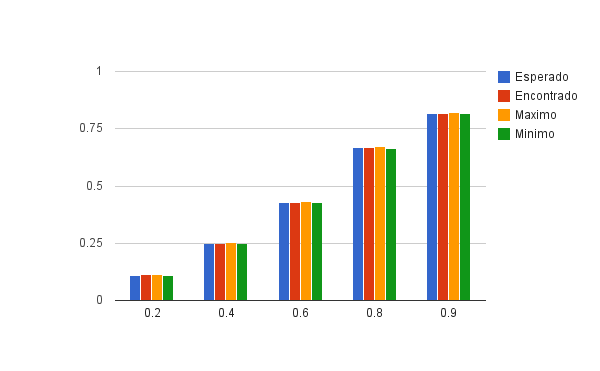
\includegraphics[scale=0.7]{E[W1].png}
    \caption{Gráfico de E[W1]}
\end{figure}
\newpage

\item \textbf{Gráfico de E[Nq1]}
\begin{table}[H] 
	      \scalefont{0.7}
	      \begin{tabular}{|c|c|c|c|c|}
		    \hline
		    $\rho$	&Esperado		&Encontrado		&Maximo			&Minimo			\\ \hline
		    0.2		&0.011111111111111	&0.011209642970553	&0.011338986172909	&0.011080299768198	\\ \hline
		    0.4		&0.05			&0.050008211402201	&0.050413364777661	&0.04960305802674	\\ \hline
		    0.6		&0.12857142857143	&0.12877350638152	&0.12981185823908	&0.12773515452396	\\ \hline
		    0.8		&0.26666666666667	&0.26723775639467	&0.26914182756829	&0.26533368522106	\\ \hline
		    0.9		&0.36818181818182	&0.36775387729734	&0.3690461140906	&0.36646164050408	\\ \hline
	      \end{tabular}
	      \caption{valores de E[Nq1]}   
\end{table}
\begin{figure}[H]
    \center
    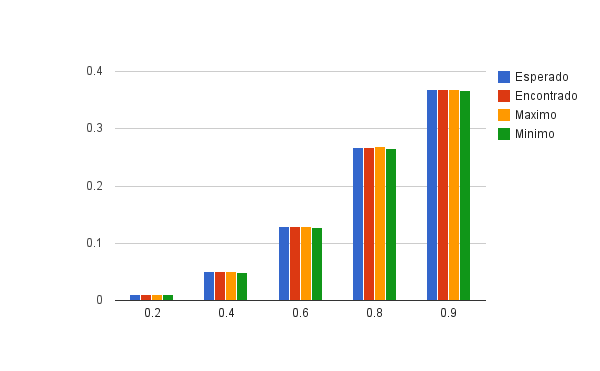
\includegraphics[scale=0.7]{E[Nq1].png}
    \caption{Gráfico de E[Nq1]}
\end{figure}

\newpage

\item \textbf{Gráfico de E[T1]}
\begin{table}[H] 
	      \scalefont{0.7}
	      \begin{tabular}{|c|c|c|c|c|}
		    \hline
		    $\rho$	&Esperado		&Encontrado		&Maximo			&Minimo			\\ \hline
		      0.2	&1.11111111111111	&1.11351613947233	&1.11584068356874	&1.11119159537592	\\ \hline
		      0.4	&1.25			&1.24873086883092	&1.25190036009894	&1.2455613775629	\\ \hline	
		      0.6	&1.42857142857143	&1.42820652048646	&1.43243881748345	&1.42397422348947	\\ \hline
		      0.8	&1.66666666666667	&1.66757154267597	&1.6722867741044	&1.66285631124753	\\ \hline
		      0.9	&1.81818181818182	&1.81716278011947	&1.82029417447625	&1.8140313857627	\\ \hline
	      \end{tabular}
	      \caption{valores de E[T1]}
\end{table}
\begin{figure}[H]
    \center
    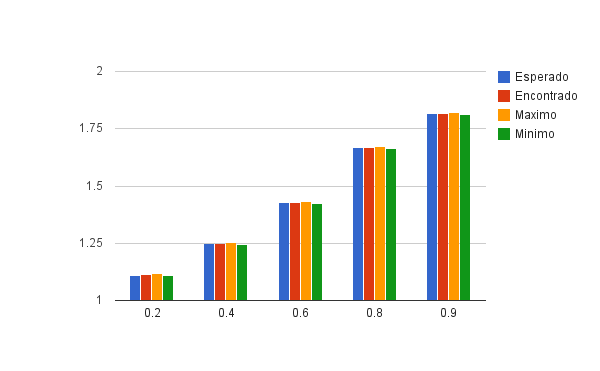
\includegraphics[scale=0.7]{E[T1].png}
    \caption{Gráfico de E[T1]}
\end{figure}

\newpage

\item \textbf{Gráfico de E[N1]}
\begin{table}[H] 
	      \scalefont{0.7}
	      \begin{tabular}{|c|c|c|c|c|}
		    \hline
		    $\rho$	&Esperado		&Encontrado		&Maximo			&Minimo			\\ \hline
		    0.2		&0.11111111111111	&0.11124715990523	&0.11156826408472	&0.11092605572575	\\ \hline
		    0.4		&0.25			&0.24971283790112	&0.25053203271413	&0.2488936430881	\\ \hline
		    0.6		&0.42857142857143	&0.42857279925318	&0.43021549392611	&0.42693010458026	\\ \hline
		    0.8		&0.66666666666667	&0.66712860751545	&0.66956348617731	&0.66469372885358	\\ \hline
		    0.9		&0.81818181818182	&0.81777623631782	&0.81932513062072	&0.81622734201492	\\ \hline	
	      \end{tabular}
	      \caption{valores de E[N1]}
\end{table}
\begin{figure}[H]
    \center
    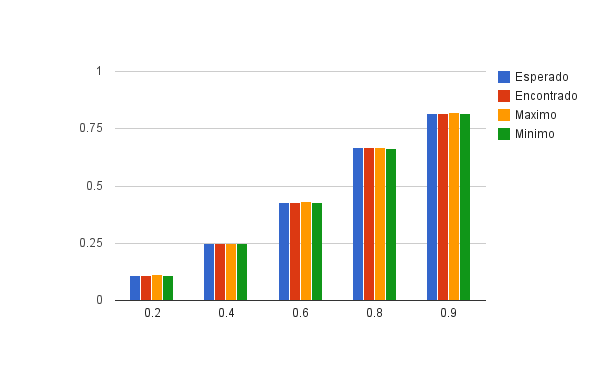
\includegraphics[scale=0.7]{E[N1].png}
    \caption{Gráfico de E[N1]}
\end{figure}

\newpage

\item \textbf{Gráfico de E[W2]}
\begin{table}[H] 
	      \scalefont{0.7}
	      \begin{tabular}{|c|c|c|c|c|}
		    \hline
		    $\rho$	&Esperado		&Encontrado		&Maximo			&Minimo			\\ \hline
		      0.2	&0.52777777777778	&0.52872616965278	&0.53281299637416	&0.52463934293141	\\ \hline
		      0.4	&1.5			&1.50022751178363	&1.51436135926444	&1.48609366430282	\\ \hline
		      0.6	&3.64285714285714	&3.63072742608245	&3.66827410034753	&3.59318075181737	\\ \hline
		      0.8	&10.6666666666667	&10.6745457878966	&10.816718996599	&10.5323725791942	\\ \hline
		      0.9	&25.3636363636364	&25.2799700922782	&25.5654287666901	&24.9945114178663	\\ \hline	
	      \end{tabular}
	      \caption{valores de E[W2]}
\end{table}
\begin{figure}[H]
    \center
    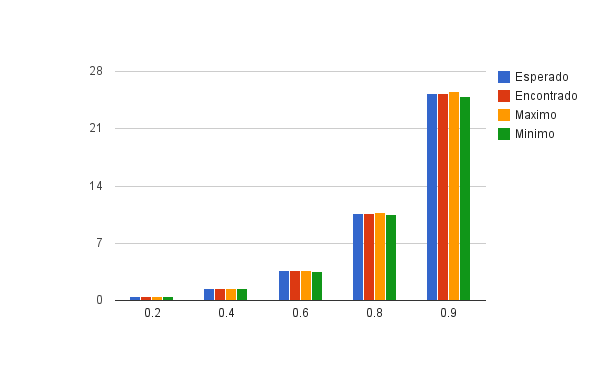
\includegraphics[scale=0.7]{E[W2].png}
    \caption{Gráfico de E[W2]}
\end{figure}

\newpage

\item \textbf{Gráfico de E[Nq2]}
\begin{table}[H] 
	      \scalefont{0.7}
	      \begin{tabular}{|c|c|c|c|c|}
		    \hline
		    $\rho$ 	&Esperado		&Encontrado		&Maximo			&Minimo			\\ \hline
		      0.2	&0.052777777777778	&0.052824522969304	&0.053261358014342	&0.052387687924266	\\ \hline
		      0.4	&0.3			&0.30003697635306	&0.30318335060684	&0.29689060209928	\\ \hline
		      0.6	&1.09285714285714	&1.08960654437444	&1.10194242488134	&1.07727066386753	\\ \hline
		      0.8	&4.26666666666667	&4.2708480816448	&4.33075721326658	&4.21093895002301	\\ \hline
		      0.9	&11.4136363636364	&11.3770691373038	&11.5082143124492	&11.2459239621583	\\ \hline
	      \end{tabular}
	      \caption{valores de E[Nq2]}
\end{table}
\begin{figure}[H]
    \center
    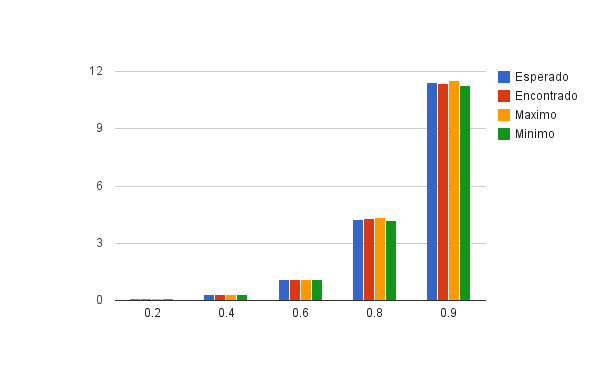
\includegraphics[scale=0.7]{E[Nq2].png}
    \caption{Gráfico de E[Nq2]}
\end{figure}

\newpage

\item \textbf{Gráfico de E[T2]}
\begin{table}[H] 
	      \scalefont{0.7}
	      \begin{tabular}{|c|c|c|c|c|}
		    \hline
		    $\rho$ 	&Esperado		&Encontrado		&Maximo			&Minimo			\\ \hline
		      0.2	&1.52777777777778	&1.52967803675752	&1.53461548194256	&1.52474059157249	\\ \hline
		      0.4	&2.5			&2.50038721593718	&2.51503307611335	&2.48574135576101	\\ \hline
		      0.6	&4.64285714285714	&4.62946384570244	&4.66733109497981	&4.59159659642506	\\ \hline
		      0.8	&11.6666666666667	&11.6742186334784	&11.8168127976126	&11.5316244693442	\\ \hline
		      0.9	&26.3636363636364	&26.2800652018098	&26.565792938344	&25.9943374652756	\\ \hline
	      \end{tabular}
	      \caption{valores de E[T2]}
\end{table}
\begin{figure}[H]
    \center
    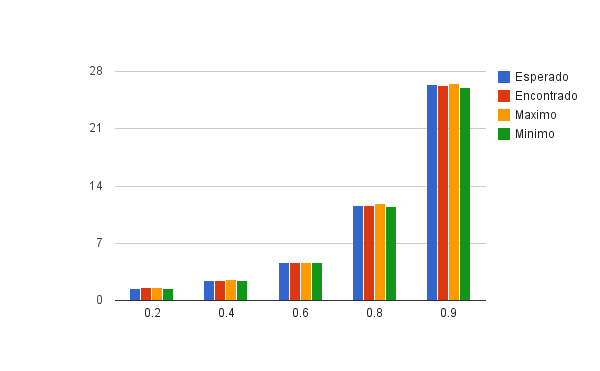
\includegraphics[scale=0.7]{E[T2].png}
    \caption{Gráfico de E[T2]}
\end{figure}

\newpage

\item \textbf{Gráfico de E[N2]}
\begin{table}[H] 
	      \scalefont{0.7}
	      \begin{tabular}{|c|c|c|c|c|}
		    \hline
		    $\rho$ 	&Esperado		&Encontrado		&Maximo			&Minimo			\\ \hline
		      0.2	&0.15277777777778	&0.15282537790103	&0.15342712044192	&0.15222363536013	\\ \hline
		      0.4	&0.5			&0.50004367176965	&0.50354770117085	&0.49653964236844	\\ \hline
		      0.6	&1.39285714285714	&1.38930100881724	&1.40206438039037	&1.37653763724412	\\ \hline
		      0.8	&4.66666666666667	&4.67076649463562	&4.73112982696196	&4.61040316230929	\\ \hline
		      0.9	&11.8636363636364	&11.8271401332377	&11.9585143917964	&11.695765874679	\\ \hline
	      \end{tabular}
	      \caption{valores de E[N2]}
\end{table}
\begin{figure}[H]
    \center
    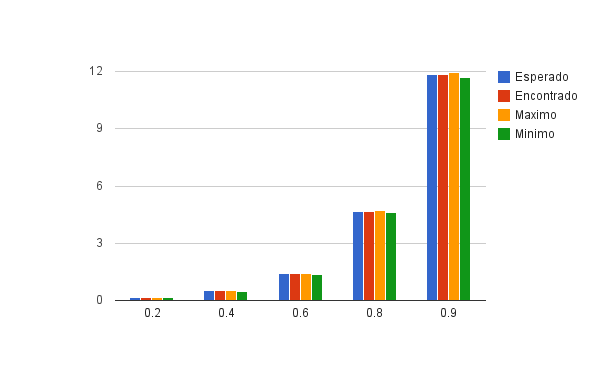
\includegraphics[scale=0.7]{E[N2].png}
    \caption{Gráfico de E[N2]}
\end{figure}
\newpage

      \end{itemize}
      \subsection{Otimização}
      \subsection{Conclusão}
      \subsection{Anexo}
      Foi gerado como parte da documentação do programa o Javadoc, é um gerador de documentação criado pela Sun Microsystems para documentar a API dos programas em Java, a partir do código-fonte.
      O resultado é expresso em HTML. É constituído, basicamente, por algumas marcações muitos simples inseridas nos comentários do programa.

      Estrutura interna da pasta Trabalho\_Final\_MAB515 , e um explicação do que econtramos nela:
      \begin{table}[H] 
	   \scalefont{0.7}
	   \begin{tabular}{|c|c|}
		   \hline   
		    doc           & Pasta onde está localizado o Javadoc.		\\ \hline
		    Relatório     & Onde se econtra o relatório do programa.		\\ \hline
		    Simulador     & Nela encontramos dentro da pasta src o código.	\\ \hline
		    Simulador.jar & arquivo que contém todas as classes compactadas , para poder executar o simulador.	\\ \hline
		    simulador.bat & arquivo que servirá para executar o comando para inicializar o servidor.Funciona apenas no windows.	\\ \hline
		    simulador.sh  & arquivo que servirá para executar o comando para inicializar o servidor.Funciona apenas no Linux.	\\ \hline
		    XML           & Onde se econtra o config.xml para quando rodar o simulador.jar, ele poder ler este arquivo.	\\ \hline
		    
	   \end{tabular}
      \end{table}
      Segue abaixo uma explicação superfícial do que as classes e seus metódos fazem, para obter melhores informações sobre os métodos, como qual são seus parâmetros o que retornam vá ao javadoc que lá irá encontrar tudo mais explicado.
      O programa está dividido em quatro pacotes.
      \begin{itemize}
	  \item br.ufrj.dcc.controle
	      \begin{itemize}
		\item \textbf{GeradorAleatorio.java\\}
		      Classe que gera as amostras do sistema.
		    \begin{itemize}
			\item \textit{GeradorAleatorio\\}
			 Construtor da classe neste caso é private, porque implementamos o padrão de projeto singleton, que faz com que haja apenas uma instância deste objeto no sistema.
			\item \textit{getInstance\\} 
			  Retorna a instância desta classe, quando este método é chamado pela primeira vez será criada a mesma.  
			\item \textit{getGeraAmostra\\}
			  Gera uma amostra usando a fórmula $x_0 = -\frac{\ln u_0}{taxa}$ , onde a taxa é passada como parâmetro.
		    \end{itemize}
		\item \textbf{GerenciadorEventos.java\\}
			 Classe que gerência os eventos do programa que podem ser chegada ou sada ou interrupção.
		     \begin{itemize}
			\item \textit{geraEventoSaida\\}
			 Método que gera um evento de saida do sistema ou seja pedo um freguês de uma das duas filas e coloco em serviço.
			\item \textit{geraEventoChegada\\}
			 Gera um evento de chegada ou seja um cliente chegando a fila 1.
			\item \textit{geraEventoDeInterrupcao\\}
			  Sempre é chamado quando ocorre um evento de chegada e quem está em serviço é um freguês oriundo fa fila2 , com isso tiramos o cliente em serviço e devolvemos a sua fila e pegamos o novo cliente em 
			  e colocamos no servidor.
			\item \textit{pegarProximoEvento\\}
			  Pega o próximo evento a ser tratado de acordo com sua hora de ocorrência,os eventos podem ser de chegada ou saida.
			\item \textit{getProximoEventoSaida\\}
			  Retorna o próximo evento de saida.
		    \end{itemize}
		\item \textbf{ManipulaXML.java\\}
		      Classe que realiza a leitura do config.xml
		     \begin{itemize}
			 \item \textit{ManipulaXML\\} 
			  Construtor da classe que recebe como parâmetro o caminho do arquivo , como padrão está o diretório do projeto na pasta XML.
			 \item \textit{leConfiguracao\\} 
			  Abre o arquivo e começa a ler as tags.
			 \item \textit{getChildTagValue\\}
			  Recebe como parâmetro o nome da tag e retorna o seu valor.
		    \end{itemize}
		\item \textbf{Rodada.java\\}
		    Classe que realiza a rodada
		    \begin{itemize}
			\item \textit{Rodada\\}
			Construtor da Classe recebe como parâmetro um objeto da classe de Configuração e Resultado, para poder verficar os parâmetros para cada rodada e amarzenar o resultado de cada rodada.
			\item \textit{simulacao\\}   Realiza efetivamente a rodada nela crio as filas de acordo com disciplina de atendimento informada, a partir dai começa-se a gerar chagadas no sistema.
		    \end{itemize}
		\item \textbf{Simulador.java\\}
		    Classe que é chamada ao iniciar o sistema.
		    \begin{itemize}
			\item \textit{main\\}Primeiro método a sere chamado assim que o programa é iniciado , nele criamos um "loop" de acordo com a quantidade de rodadas que serão feitas para após 
					     retornar os resultados estatísticos.
			\item \textit{calculaIntervaloDeConfianca\\}Realiza o cálculo do intervalo de confiança fazendo uso da T-Student como o valor de $1.96$ , o que nos dá uma precisão de 95\%.
			\item \textit{calculaMedia\\} Realiza o cálculo da média para exbir a reposta , fazendo uso do valor médio obtido em cada rodada.
		    \end{itemize}
	     \end{itemize}
	\item br.ufrj.dcc.modelo
	   \begin{itemize}
	      \item \textbf{Configuaracao.java\\}
		    Armazena os parâmetros que serão utilizados na simulação.
		    \begin{itemize}
			 \item  \textit{Configuracao\\}
			 Construtor da classe recebe como parâmetro os seguintes valores: fase transiente, número  de rodadas,tamanho das rodadas,taxa de serviço , utilização e a disciplina de atendimento
			 das duas filas.
			 \item  \textit{getFaseTransiente\\}
			  Retorna a quatidade de clientes que pertecem a fase transiente.
			 \item  \textit{getNumeroRodada\\}
			  Retorna o número de rodadas que iermos fazer.
			 \item  \textit{getTamanhoRodada\\}
			  Retorna a quantidade de eventos de chegada que iremos gerar.
			 \item  \textit{getTaxaServico\\}
			  Retorna a taxa de serviço do servidor.
			 \item  \textit{getUtilizacao\\}
			  Retorna a utilização do sistema.
			 \item  \textit{getFila1\\}
 			  Retorna a disciplina de atendimento da fila1
			 \item  \textit{getFila2\\}
% 			  Retorna a discilina de atendimento da fila2
		    \end{itemize}
	      \item \textbf{Evento.java\\}
		     Classe que armazena os valores especificados no xml.
		    \begin{itemize}
			 \item  \textit{Evento\\}
			  Construtor nesta classe temos dois ,quando passamos como parâmetro um frêgues indica que estamos criando um  evento de chegada caso seja o servidor estamos criando um evento de Saida. 
			 \item  \textit{isEventoChegada\\}
			  Retorna true se o evento é de chegada	.		  
			 \item  \textit{isEventoSaida\\}
 			  Retorna true se o evento é de saida.
			 \item  \textit{getFregues\\}
			  Retorna o freguês que gerou o evento , apenas utilizado se for de chegada.
			 \item  \textit{getTipo\\}
 			  Retorna o tipo do evento que pode ser de chegada ou saida.
			 \item  \textit{getHoraOcorrencia\\}
			  Retorna a hora que irá ocorrer o evento.
			 \item  \textit{getServer\\}
			  Retorna o servidor ao qual iremos colocar o freguês, apenas utilizado para evento de saida.			  
		    \end{itemize}
	      \item \textbf{Fregues.java\\}
		    Classe que faz o papel de um freguês no sistema.
		    \begin{itemize}
			 \item  \textit{setCor\\}indentifica se o cliente pertence a fase transiente.
			 \item  \textit{getCor\\}Retorna o valor do campo que unicamente pode ser preenchido com "TRANSIENTE" ou "NAOTRANSIENTE".
			 \item  \textit{setInstanteChegadaFila1\\}Preenche a variável que indica quando o cliente chegou no sistema e entrou na fila1.
			 \item  \textit{getInstanteChegadaFila1\\}Retorna o valor da variável.
			 \item  \textit{setInstanteSaidaFila1\\}Preenche a variável que indica quando o cliente saiu da fila1 e foi para o servidor.
			 \item  \textit{getInstanteSaidaFila1\\}Retorna o valor da variável.
			 \item  \textit{setInstanteChegadaFila2\\}Preenche a variável que indica quando o instante de chegada do cliente a fila 2.
			 \item  \textit{getInstanteChegadaFila2\\}Retorna o valor da variável.
			 \item  \textit{setInstanteSaidaFila2\\}Preenche a variável que indica momento em que saiu da fila2 e foi para o servidor.
			 \item  \textit{getInstanteSaidaFila2\\}Retorna o valor da variável.
			 \item  \textit{setInstanteSaidaSistema\\}Preenche a variável que indica momento em que acabou de ser servido e pode ir embora do sistema
			 \item  \textit{getInstanteSaidaSistema\\}Retorna o valor da variável.
			 \item  \textit{setServicoResidual\\}Preenche a variável que indica caso o tempo falta para acabar de ser servido.Este campo é preenchido quando ocorre uma interrupção.
			 \item  \textit{getServicoResidual\\}Retorna o valor da variável.
			 \item  \textit{setFilaOrigem\\}Preenche a variável que indica para o que faremos com o frêgues após ser servido se pode ir embora ou o colocamos na fila2.
			 \item  \textit{getFilaOrigem\\}Retorna o valor da variável.
			 \item  \textit{chegarNoSistema\\}Preencha as variáveis necessárias como instante de chegada na fila, e inseri o novo 
		    \end{itemize}
	      \item \textbf{Resultado.java\\}
		    Classe que armazena o resultado de cara Rodada.
		    \begin{itemize}
			 \item  \textit{getT1\\}Retorna um "array" com tempo total médio de que um freguês levou para sair do sistema 1(sair da fila mais acabar ser ser servido), de cada rodada.  
			 \item  \textit{getT2\\}Retorna um "array" com tempo total médio de que um freguês levou para sair do sistema 2(sair da fila mais acabar ser ser servido), de cada rodada.  
			 \item  \textit{getW1\\}Retorna um "array" com tempo de espera médio de um cliente na fila1, de cada rodada.
			 \item  \textit{getW2\\}Retorna um "array" com tempo de espera médio de um cliente na fila2, de cada rodada.
			 \item  \textit{getN1\\}Retorna um "array" com número médio de clientes que passaram pela fila1, de cada rodada. 
			 \item  \textit{getN2\\}Retorna um "array" com número médio de clientes que passaram pela fila2, de cada rodada.
			 \item  \textit{getNq1\\}Retorna um "array" com o número médio de fregueses que ficaram esperando na fila 1, de cada rodada.
			 \item  \textit{getNq2\\}Retorna um "array" com o número médio de fregueses que ficaram esperando na fila 2, de cada rodada.
			 \item  \textit{getVarianciaW1\\}Retorna um "array" com a variância do tempo de espera médio na fila1  em acada rodada.
			 \item  \textit{getVarianciaW2\\}Retorna um "array" com a variância do tempo de espera médio na fila2  em acada rodada.
			 \item  \textit{setT1\\}adiciona ao "array" o tempo total médio de que um freguês levou para sair do sistema 1(sair da fila mais acabar ser ser servido) na última rodada.
			 \item  \textit{setT2\\}adiciona ao "array" o tempo total médio de que um freguês levou para sair do sistema 2(sair da fila mais acabar ser ser servido) na última rodada.
			 \item  \textit{setW1\\}adiciona ao "array" o tempo de espera médio de um cliente na fila1 na última rodada.
			 \item  \textit{setW2\\}adiciona ao "array" o tempo de espera médio de um cliente na fila2 na última rodada.
			 \item  \textit{setN1\\}adiciona ao "array" o número médio de clientes que passaram pela fila1 na última rodada.
			 \item  \textit{setN2\\}adiciona ao "array" o número médio de clientes que passaram pela fila2 na última rodada.
			 \item  \textit{setNq1\\}adiciona ao "array" o número médio de fregueses que ficaram esperando na fila 1 na última rodada.
			 \item  \textit{setNq2\\}adiciona ao "array" o número médio de fregueses que ficaram esperando na fila 2 na última rodada.
			 \item  \textit{setVarianciaW1\\}adiciona ao "array" a variância do tempo de espera médio na fila1  na última rodada.
			 \item  \textit{setVarianciaW2\\}adiciona ao "array" a variância do tempo de espera médio na fila2  na última rodada.
		    \end{itemize}
	      \item \textbf{Servidor.java\\}
		    Classe que faz o papel do servidor do sistema.
		    \begin{itemize}
			 \item  \textit{tempoServico\\}
                            Manda o gerador aleatório gerar uma amostrar que indica quanto tempo o cliente levará em serviço.                            
			 \item  \textit{isOcioso\\}Retorna true se não tem niguém em serviço.
			 \item  \textit{getFregues\\}Retorna o freguês que está em serviço.                            
			 \item  \textit{getFilaOrigem\\}Retorna a fila de origem do cliente que está em serviço.
			 \item  \textit{finish\\}Método que verifica se tem alguém para ser servido na fila1 ou fila2  e realiza o termino do serviço do cliente atual.
			 \item  \textit{servicoCompleto\\}Este metódo decide o que faço com o cliente que acabou de ser servido se coloco na fila 2 ou se pode ir embora do sistema.
			 \item  \textit{trataInterrupcao\\}Método que trata interrupção ou seja coloca o novo cliente em serviço , coloca o antigo na sua fila e preenche o tempo de serviço residual.
			 \item  \textit{geraResultado\\}gera o resultado da última rodada.
			 \item  \textit{getResultado\\}retorna o resultado da última rodada.
		    \end{itemize}
	   \end{itemize}
	  \item br.ufrj.dcc.modelo.enumerator
	    \begin{itemize}
		\item \textbf{CorCliente.java\\} enumerator criado para representar as possíveis cores que um cliente pode assumir, como no nosso caso estamos usando o método replicativo só podem ser duas "TRANSIENTE" ou "NAOTRANSIENTE".
		\item \textbf{FilaOrigem.java\\} enumerator criado para localizar aonde os freguês se encontra no sistema:"FILA1" e "FILA2".
		\item \textbf{TipoEvento.java\\} enumerator criado para destacar apenas os eventos gerados no sistema que são: "SAIDA" e "CHEGADA".
	     \end{itemize}
	  \item br.ufrj.dcc.modelo.fila
	      \begin{itemize}
		\item \textbf{Fila.java\\} É uma super\-classe da FCFS e LCFS, utilizamos ela para não precisar implementar todos os metódos duas vezes apenas os que são direntes em cada disciplina de atendimento. 
		    \begin{itemize}
			 \item \textit{Fila \\} Está classe também possui dois construtors, um para a fila 1 que recebe como parâmetro o servidor, $\lambda$ que é taxa com que os freguese chegam ao sistema como também a fila 2,
						a qual tenho mais prioridada  e outro para a fila2 pois nela não ocorrem chegadas e nem é mais prioritária que outra fila , dessa forma só recebe o serviço.
			 \item \textit{removeParaAtendimento\\} deve ser implementado pela classe que herda dessa.
			 \item \textit{addFregues\\} deve ser implementado pela classe que herda dessa.
			 \item \textit{addFreguesResidual\\} deve ser implementado pela classe que herda dessa.
			 \item \textit{calculaProximaChegada\\} Manda o gerador aleatório gerar uma amostrar que indica quando irá chegar um cliente no sistema.
			 \item \textit{isEmpty\\} Retorna true se a fila está vazia.
			 \item \textit{size\\} Retorna o tamanho da fila no istante que este metódo é chamado.
			 \item \textit{getNumeroTotalChegadas\\}Retorna a quantidade de pessoas que já passaram pela fila.
			 \item \textit{getLambda \\}Retorna a taxa de chegada, que no caso da fila1 será o valor de $\lambda$, já na fila2 será $0.0$
		    \end{itemize}
		\item \textbf{FCFS.java\\}
		    \begin{itemize}
			 \item \textit{FCFS \\}Crio objeto do tipo FCFS e recebe os parâmetros e passa para a super-classe.
			 \item \textit{removeParaAtendimento\\} Retorna o primeiro freguês da fila para ser atendido.
			 \item \textit{addFregues\\} Adiciona o cliente que acabou de chegar ao final da fila.
			 \item \textit{addFreguesResidual \\} Inseri o cliente que possui resíduo ou seja que sofreu um interrupção no íncio da fila.			  
		    \end{itemize}
		\item \textbf{LCFS.java\\}
		    \begin{itemize}
			 \item \textit{LCFS \\}Crio objeto do tipo FCFS e recebe os parâmetros e passa para a super-classe.
			 \item \textit{removeParaAtendimento\\}Retornat  o primeiro freguês da pilha para ser atendido
			 \item \textit{addFregues\\}Adiciona o cliente que acabou de chegar no inicio da fila.
			 \item \textit{addFreguesResidual \\} Inseri o cliente que possui resíduo ou seja que sofreu um interrupção no íncio da fila.			  
		    \end{itemize}
	     \end{itemize}
      \end{itemize}
\end{document}

